%
% File acl2015.tex
%
% Contact: car@ir.hit.edu.cn, gdzhou@suda.edu.cn
%%
%% Based on the style files for ACL-2014, which were, in turn,
%% Based on the style files for ACL-2013, which were, in turn,
%% Based on the style files for ACL-2012, which were, in turn,
%% based on the style files for ACL-2011, which were, in turn,
%% based on the style files for ACL-2010, which were, in turn,
%% based on the style files for ACL-IJCNLP-2009, which were, in turn,
%% based on the style files for EACL-2009 and IJCNLP-2008...

%% Based on the style files for EACL 2006 by
%%e.agirre@ehu.es or Sergi.Balari@uab.es
%% and that of ACL 08 by Joakim Nivre and Noah Smith

\documentclass[11pt]{article}
\usepackage[utf8]{inputenc}
\usepackage[T1]{fontenc}
\usepackage{acl2015}
\usepackage[backend=biber,
            style=authoryear-icomp,
            doi=false,
            isbn=false,
            url=false,
            maxcitenames=1]{biblatex}
\usepackage{times}
\usepackage{url}
\usepackage{latexsym}% -*- program: Value -*-
\usepackage{graphicx}
\usepackage[colorlinks=false, pdfborder={0 0 0}]{hyperref}
\usepackage[noabbrev, nameinlink]{cleveref}
\usepackage{booktabs}
\usepackage{adjustbox}
\usepackage{pgfplots}
\pgfplotsset{width=\columnwidth,compat=1.10}

\def\labelitemi{--}

\addbibresource{bibliography.bib}
%\setlength\titlebox{5cm}

% You can expand the titlebox if you need extra space
% to show all the authors. Please do not make the titlebox
% smaller than 5cm (the original size); we will check this
% in the camera-ready version and ask you to change it back.


\title{POS Driven Cross-Lingual Pronoun Prediction with Feed-Forward Neural Networks}

\author{Jimmy Callin \\
  Uppsala University \\
  {\tt jimmy.callin@gmail.com}}

\date{}

\begin{document}
\maketitle
\begin{abstract}
    For some language pairs, pronoun translation is a discourse driven task. For cross-lingual pronoun prediction, we suggest a neural network based model using preceding nouns and determiners as features for suggesting antecedent candidates. Our model scores on par with similar models while having a simpler architecture.
\end{abstract}


\section{Introduction}

Translation requires context.
Most modern statistical machine translation (SMT) systems do use context for translation; the meaning of a word is more often than not ambiguous, and can only be decoded through its usage.
That said, context in modern SMT still mostly assumes that sentences are independent of each other, and sentence dependencies are simply ignored.
While today's popular SMT systems could and in some cases do use source language features from previous sentences, previously translated sentences within a document has up to this point rarely been included.
\textcite{Hardmeier2010Modelling} argue that SMT research has become mature enough to stop assuming sentence independence, and start to incorporate features beyond the sentence boundary.
They demonstrate the difficulty of correctly determining the correct German pronoun given English as source language.
While translating pronouns indeed can be unproblematic for certain language pairs, languages with gender-marked pronouns introduce certain difficulties, since the choice of pronoun is determined upon the gender of its antecedent.
Picking the wrong third-person pronoun might seem like a relatively minor error, especially if present in an otherwise comprehensible translation, but could potentially produce misunderstandings. Take the following English sentences:

\begin{itemize}
    \setlength{\itemsep}{-0.2em}
    \item The monkey ate the banana because \emph{it} was hungry.
    \item The monkey ate the banana because \emph{it} was ripe.
    \item The monkey ate the banana because \emph{it} was tea-time.
\end{itemize}

\emph{It} in each of these three cases reference something different, either the monkey, the banana, or the abstract notion of time. If we were to translate these sentences to German, we would have to consciously make decisions whether \emph{it} should be in masculine (\emph{der}, referring to the monkey), feminine (\emph{die}, referring to the banana), or neuter (\emph{das}, referring to the time) (\cite{Mitkov1995Anaphora}). While these examples use a local dependency, the antecedent of \emph{it} could just as easily have been one or several sentences away and its translation would have been out of reach for sentence based SMT decoders.


\section{Related work}


Most of the work in anaphora resolution for machine translation has been done in the paradigm of rule-based MT, while the topic has gained little interest within SMT (\cite{Hardmeier2010Modelling, Mitkov1999Introduction}).
One of the first examples of using discourse analysis for pronoun translation in SMT was done by \textcite{Nagard2010Aiding}, where they use co-reference resolution to predict the antecedents in the source language as features in a standard SMT system.
While they saw score improvements in pronoun prediction, the bad performance of the co-reference resolution seriously impacts the results negatively.
They implement this in a two-step solution by running the co-reference resolver separately from the SMT decoder, and thereafter annotate the translated French pronouns with gender and quantity based on their predicted antecedent from which they once again translate using another MT system where phrase tables have been annotated in the same fashion.
This seems to be mostly for practical reasons, since most popular SMT frameworks such as Moses do not provide previous target translations for use as features (\cite{Koehn2007Moses}).
\textcite{Guillou2012Improving} tries a similar approach for English-Czech translation with little improvement even after factoring out major sources of error. They single out one possible reason for this, which is how a reasonable translation alternative of a pronoun's antecedent could affect the predicted pronoun, including the possibility of simply canceling out pronouns. E.g, \emph{the u.s. , claiming some success in its trade} could be paraphrased as \emph{the u.s. , claiming some success in trade diplomacy} without any loss in translation quality, while still affecting the score negatively.

In reality, there is necessary linguistic information in the target translation that simply is not available in the source.
An English antecedent might in most cases be translated to a word with male gender, which is learned by the decoder.
This means that in cases where the antecedent produce an alternative translation with a non-male gender, the decoder has no information available to condition upon this.
It could potentially be possible to include a larger source context window around the source antecedent in hope of catching contexts where alternative translations are made, but in our opinion this would likely only increase data sparseness and overall be a non-optimal solution.
Rather, you would like to have the translated antecedent available at decoding, which would mean that the SMT decoder in contrast to most decoders today should be able to handle dependencies across sentence boundaries.
\textcite{Hardmeier2010Modelling} extends the phrase-based Moses decoder with a word dependency model based on existing co-reference resolution systems, by parsing the output of the decoder and catching its previous translations.
Unfortunately they only produce minor improvements for English-German, and negative results for English-French (\cite{Hardmeier2011UppsalaFbk}).

In light of this, there have been attempts at considering pronoun translation as a classification task separate from traditional machine translation.
This could  could potentially lead to further insights into the nature of anaphora resolution.
In this fashion a pronoun translation module could potentially be treated as just another part of translation by discourse oriented machine translation systems, or as a post-processing step similarly to \textcite{Guillou2012Improving}.
\textcite{Hardmeier2013Latent} introduce this task and present a feed-forward neural network model using features from an external anaphora resolution system, BART (\cite{Broscheit2010Bart}), to infer the pronoun's antecedent candidates and use the aligned words in the target translation as input. This model is later integrated into their document-level decoder Docent (\cite[chapter~9]{Hardmeier2014Discoursea}; \cite{Hardmeier2013Docent}).

\section{Task setup}

The goal of this task is to accurately predict the correct pronoun in a French translation.
The pronouns in focus are \emph{she}, \emph{he}, \emph{it}, and \emph{they}, where the word aligned phrases in the French translation have been replaced by placeholders.
The word alignment is included, and was automatically produced by GIZA++ (\cite{Och2003Giza}).
We are also aware of document boundaries within the corpus.
The corpus is a set of three different parallel corpora gathered from three separate domains:
transcribed TED talks, Europarl (\cite{Koehn2005Europarl}) with transcribed proceedings from the European parliament, and a set of news text.
Test data is a collection of transcribed TED talks, in total 12 documents containing 2093 sentences with a total of 1105 classification problems, with a similar development set.

\section{Method}

Inspired by the the neural network architecture set up in \textcite{Hardmeier2013Latent}, we similarly propose a feed-forward neural network with a layer of word embeddings as well as an additional hidden layer for learning abstract feature representations.
The model is trained using stochastic gradient descent with mini-batches and L2 regularization.
Cross-entropy is used as a cost function, with a softmax output layer.
The main difference in our model lies in avoiding using antecedent features as gathered by an external anaphora resolution system.
Rather, to simplify the model we try to simply look at the four closest previous nouns and determiners in English, and use the corresponding aligned French nouns and articles in the model, as illustrated in \cref{fig:posexample}.
Wherever the alignments map to more than one word, only the furthermost left of the words in the phrase is used.

\begin{figure}[htbp]
    \centering
    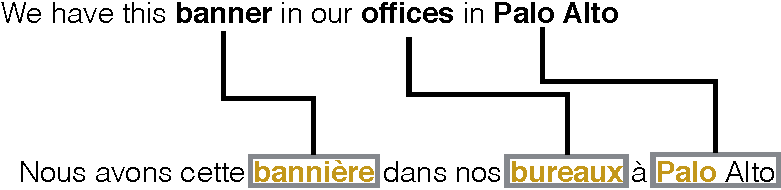
\includegraphics[width=\columnwidth]{figures/posexample.pdf}
    \caption{An English POS tagger is used to find nouns and articles in preceding utterances, while the word alignments determine which French words are to be used as features.}
    \label{fig:posexample}
\end{figure}


Additionally, we allow ourselves to look at the French context of the missing pronoun.
While this restricts the potential usage of our model as a part of the translation process, French usage should be a better indicator for some of the classes, e.g. \emph{ce} which is highly dependent being precedent of \emph{est}.
See \cref{fig:contextexample} for an example of context in source and translation as features.

\begin{figure}[htbp]
    \centering
    
\includegraphics[width=\columnwidth]{figures/contextexample.pdf}
    \caption{Example of context used in the classification model, color coded according to their position in the neural network as illustrated in \cref{fig:nnarchitecture}.}
    \label{fig:contextexample}
\end{figure}

Furthermore the dimensionality of the embeddings are increased from 20 to 50, since this was empirically shown to somewhat improve the scores on the development set, with a hidden layer size of 50.
To reduce training time and faster find convergence, we use $\tanh$ as activation function between the hidden layers, in contrast to the sigmoid function in the original paper (\cite{Lecun2012Efficient}).
To avoid overfitting, early stopping is introduced where the training stops if no improvements have been found within a number of iterations.
This usually results in a training time of 130 epochs, when run on TED data from IWSLT.

The model uses a uniform random weight initialization according to \textcite{Glorot2010Understanding}, where they show that neural network models using $\tanh$ as activation function generally perform better with an initialization within the interval $uniform[-\frac{\sqrt{6}}{\sqrt{fan_{in}+fan_{out}}},\frac{\sqrt{6}}{\sqrt{fan_{in}+fan_{out}}}]$, where $fan_{in}$ and $fan_{out}$ are number of inputs and number of hidden units respectively.

Since the model uses a fixed context window size for English and French, as well as a fixed number of preceding nouns and articles, we need to find out the optimal parameter settings. We empirically find that a parameter setting of 4+4 context window for English and French, with 3 preceding nouns and articles each perform well. \Cref{figure:parametervary} showcases how window size and number of preceding POS tags affect the performance outcome on the development set. We also looked into asymmetric window sizes, but according to \cref{figure:winasym} we noticed no improvements.

The final architecture as shown in \cref{fig:nnarchitecture} was implemented in Theano (\cite{Bergstra2010Theano}), and is publicly available on Github\footnote{\url{http://github.com/jimmycallin/whatelles}}.

\begin{figure*}[htbp]
    \centering
    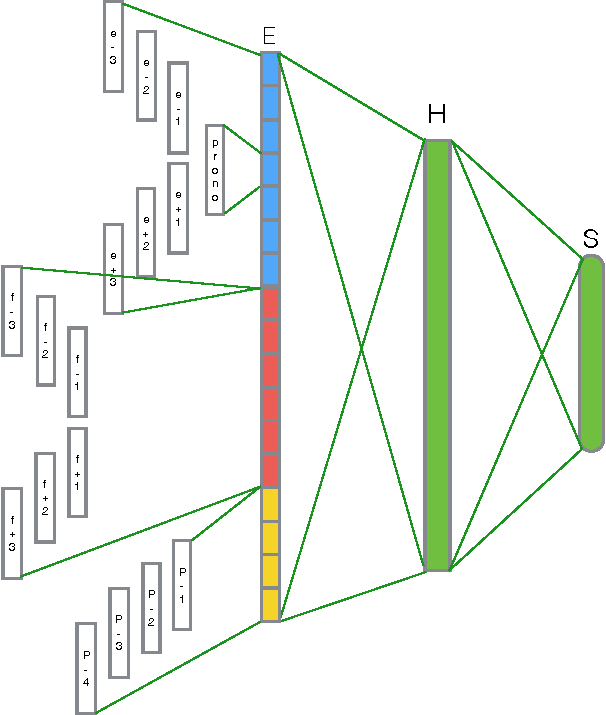
\includegraphics[width=\columnwidth]{figures/nnarchitecture.pdf}
    \caption{Neural network architecture. Blue embeddings (E) signifies source context, red target context, and yellow the preceding POS tags. The shown number of features is not equivalent with what is used in the final model.}
    \label{fig:nnarchitecture}
\end{figure*}


\begin{figure}[t]
    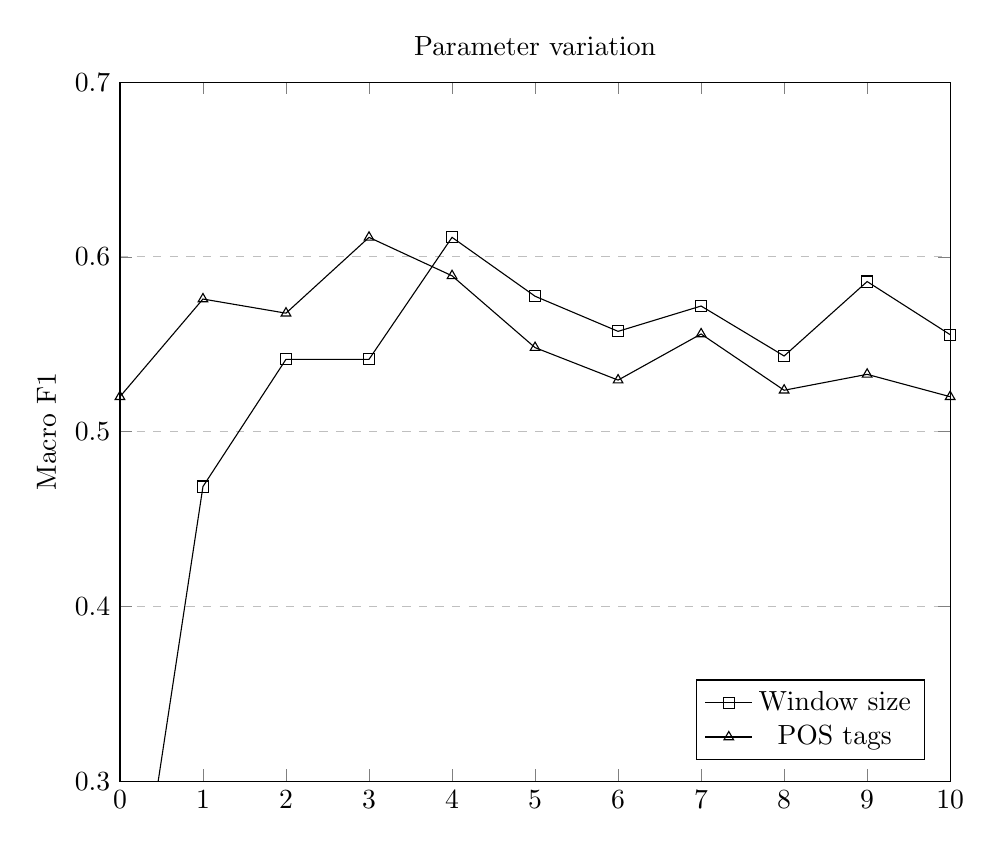
\begin{tikzpicture}
    \begin{axis}[
        title={Parameter variation},
        ylabel={Macro F1},
        xmin=0, xmax=10,
        ymin=0.3, ymax=0.7,
        xtick={0,1,2,3,4,5,6,7,8,9,10},
        ytick={0.3,0.4,0.5,0.6,0.7},
        legend pos=south east,
        ymajorgrids=true,
        grid style=dashed,
    ]
    \addplot[
        mark=square,
        ]
        coordinates {
        (0,0.1560)(1,0.4686)(2,0.5414)(3,0.5414)(4,0.6112)(5,0.5775)(6,0.5574)(7,0.5719)(8,0.5433)(9,0.5859)(10,0.5555)
        };
        \addlegendentry{Window size}

    \addplot[
        mark=triangle,
        ]
        coordinates {
        (0,0.5200)(1,0.5759)(2,0.5678)(3,0.6112)(4,0.5892)(5,0.5481)(6,0.5295)(7,0.5559)(8,0.5237)(9,0.5328)(10,0.5200)
        };

        \addlegendentry{POS tags}

    \end{axis}
    \end{tikzpicture}
\caption{Parameter variation of window size and number of preceding POS tags. Window size is varied in a symmetrical fashion of n+n. When varying window size, 3 preceding POS tags are used. When varying number of POS tags, a window size of 4+4 is used.}
\label{figure:parametervary}
\end{figure}

\begin{figure}[t]
    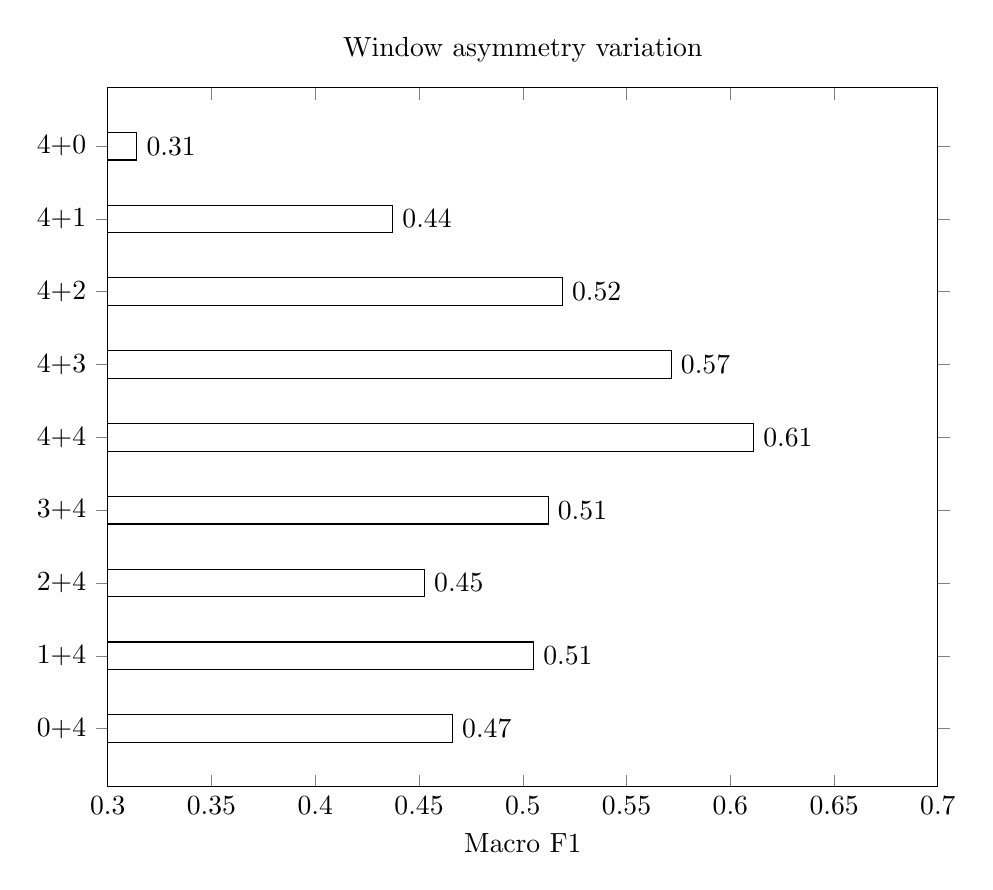
\begin{tikzpicture}
    \begin{axis}[
            title={Window asymmetry variation},
            xbar,
            xmin=0.3,
            xmax=0.7,
            ytick=data,
            xlabel={Macro F1},
            % height={ 1cm + ( 3.0 * 1cm ) },
            symbolic y coords={{0+4},{1+4},{2+4},{3+4},{4+4},{4+3},{4+2},{4+1},{4+0}},
            nodes near coords,
            nodes near coords align = {horizontal}
    ]
    \addplot[]
        coordinates {
        (0.4661,{0+4})(0.5052,{1+4})(0.4526,{2+4})(0.5122,{3+4})(0.6112,{4+4})(0.5715,{4+3})(0.5190,{4+2})(0.4373,{4+1})(0.3140,{4+0})
        };
    \end{axis}
    \end{tikzpicture}
\caption{Parameter variation of window size asymmetry, where each label corresponds to \emph{n}+\emph{n}, where \emph{n} is the context size in each direction.}
\label{figure:winasym}
\end{figure}

\section{Results}

The results from the shared task are presented in \cref{tbl:resultscores} and \cref{tbl:confmatrix}.
Best performing classes are \emph{ce}, \emph{ils}, and \emph{other}, while the less commonly occurring classes \emph{elle} and \emph{elles} have precision comparable to other classes.
Their recall, though, is significantly worse. The overall macro F1 score ends up being 55.3\%.

\begin{table}[t]
\centering
    \begin{tabular}{llll}
          & Precision & Recall  & F1      \\ \midrule
    ce    & 0.8291   & 0.8967 & 0.8616 \\
    cela  & 0.7143   & 0.6202 & 0.6639 \\
    elle  & 0.5000   & 0.2651 & 0.3465 \\
    elles & 0.6296   & 0.3333 & 0.4359 \\
    il    & 0.5161   & 0.6154 & 0.5614 \\
    ils   & 0.7487   & 0.9312 & 0.8301 \\
    other & 0.8450   & 0.8579 & 0.8514 \\
    \midrule
    Macro & 0.5816 & 0.5495 & 0.5530 \\
    Micro & 0.7213 & 0.7213 & 0.7213 \\
    \hline
    \end{tabular}
    \caption{Precision, recall, and F1-score for all classes. Micro score is the overall classification score, while macro is the average over each class. The latter scoring method is used for increasing the importance of classes with fewer instances.}
    \label{tbl:resultscores}
\end{table}

\begin{table}[t]
    \scalebox{0.8}{
    \begin{tabular*}{\columnwidth}{@{}rlllllll|l@{}}
          & ce  & cela & elle & elles & il  & ils & other & sum \\
    ce    & 165 & 3    & 0    & 1     & 8   & 1   & 6     & 184 \\
    cela  & 5   & 80   & 4    & 1     & 21  & 0   & 18    & 129 \\
    elle  & 7   & 10   & 22   & 2     & 22  & 2   & 18    & 83  \\
    elles & 0   & 0    & 0    & 18    & 0   & 31  & 3     & 51  \\
    il    & 11  & 7    & 9    & 0     & 64  & 1   & 12    & 104 \\
    ils   & 1   & 0    & 0    & 5     & 0   & 149 & 5     & 160 \\
    other & 10  & 12   & 9    & 1     & 9   & 15  & 338   & 394 \\
    \cline{1-8}
    sum   & 199 & 112  & 44   & 27    & 124 & 199 & \multicolumn{1}{l}{400}   & ~   \\
    \end{tabular*}}
    \caption{Confusion matrix of class predictions. Row signifies actual class according to gold standard, while column represents predicted class according to the classifier.}
    \label{tbl:confmatrix}
\end{table}

\section{Discussion}

Results indicate that the model performs on par with previously suggested models, while having a simpler architecture.
Classes highly dependent on local context, such as \emph{ce}, perform especially well, which is likely due to \emph{est} being a good indicator for its presence.
This is supported by the large performance gains from 4+0 to 4+1 in \cref{figure:winasym}, since \emph{est} usually follows \emph{ce}.
% il      c'      if you ask for the happiness of the remembering self , it 's a completely different thing .     si vous réfléchissez sur le bonheur du " moi des souvenirs " , REPLACE est une toute autre histoire .
Albeit, a succeeding \emph{est} is not a guarantee for the model, as shown in \emph{\_\_ est une toute autre histoire}, which it for some reason believe is a good place for \emph{il}.
Singular and plural classes rarely get mixed up, probably due to its condition upon the English pronoun which marks \emph{it} or \emph{they}, making this prediction clear.
The classes of feminine gender does not perform as well, especially not recall-wise, although this was to be expected since the only real information from which to infer its antecedent is distance from the pronoun in focus.
It is apparent that the model has a bias towards making majority class predictions, especially given the low number of wrong predictions on the \emph{elle} and \emph{elles} classes relative to \emph{il} and \emph{ils}.
The high recall of \emph{ils} is explained by this phenomenon as well.
An additional hypothesis is that it is simply too little data to realistically create usable embeddings, except for in a few reoccurring circumstances.

A somewhat interesting example of what POS tags might cause is:

\emph{... which is the history of who invented games ... and they would be so immersed in playing the dice games ...} \\
\emph{... l' histoire de qui a inventé le jeu et pourquoi ... \_\_ seraient si concentrés sur leur jeu de dés ...}

This is one of the few instances where \emph{ils} has been misclassified as \emph{elles}. Since this classification only happens when you use at least three preceding POS tags, it is likely there is something happening with the antecedent candidates. The third determiner is \emph{the (history)}, and points to \emph{histoire} which is a noun of feminine gender. It is likely the classifier has learned this connection and has put too much weight into it.

The extra number of features as well as the increase in embedding dimensionality makes the training and prediction somewhat slower, but since the training still is done in less than an hour, and predicting the test data does not take more than a few seconds, it is still good enough for general usage.
Furthermore, the implementation is made in such a way that further performance increases are to be expected if you run it on CUDA compatible GPU with minor changes.

While three separate training data collections were available, we only found interesting results when using data from the same domain as the test data, i.e. transcribed TED talks.
To overcome the skew class distribution, attempts were made at oversampling the less frequent classes from Europarl, but unfortunately this only led to performance loss on the development set.
The model does not seem to generalize well from other types of training data such as Europarl or news text, despite Europarl being transcribed speech as well.
This is an obvious shortcoming of the model.

We tried several alterations in parameter settings for context window and POS tags, and there were no significant improvements found beyond the final parameter settings when run on the development set, as seen in \cref{figure:parametervary}.
\Cref{figure:winasym} makes it clear that a symmetric window size is beneficial, while the reason for why is not made as clear.
It does seem like right context is more important than left context, which could be due to pronouns in their role as subjects largely appears early in sentences, making left context nothing but sentence start markers.
In future work, it would be interesting to look into how much source context actually contribute to the classification, given a target context.
The English context is indeed nice to have, since you cannot be entirely certain of the translation quality in the target language, but intuitively all necessary linguistic information should only be available in the target language.
If source language were to be used, each English word embedding could perhaps be pre-trained on a large number of translation examples hopefully learning the most probable cross-linguistic gender.
Gender aware French word embeddings would hypothetically increase the score as well, if not more.

\section{Conclusion}

In this work, we have been developing a cross-lingual pronoun prediction classifier based on a feed-forward neural network.
The model was heavily inspired by (\cite{Hardmeier2013Latent}), while trying to simplify the architecture by simply using preceding nouns and determiners for coreference resolution rather than using features from an anaphora extractor such as BART, as set up in the original paper, since these usually includes large performance overhead.

We find out that the model indeed perform on par with similar models, while being easier to train.
There are some expected drops in performance for the less common classes heavily dependent on finding the correct anecedent.
We discuss probable causes for this, as well as possible solutions using pretrained embeddings on larger amounts of training data.

\printbibliography
\end{document}
